\scanpage{10}
% archive sheet number: 9

a) $\Longrightarrow$ b) On voit \inserted{par polarité} que $C'$ est \deleted{\unsure{réunion}}\inserted{env.} conv. fermée d'un nb fini de pts, \deleted{et de demi-droites d'origine $0$} donc d'après ce qui précède il \deleted{donc $C'$ est \unsure{enveloppé de|enveloppe de}} est intersection finie de demi-espaces \deleted{\unsure{finie et}} fermés donc par polarité on trouve b) pour $E$, sous forme précise.

\figure{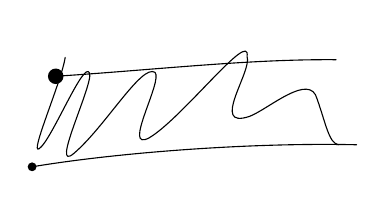
\begin{tikzpicture}[x=1cm,y=1cm,line cap=round,line join=round]
\draw (0.3,1.15) .. controls (1.55,1.23) and (2.75,1.37) .. (3.86,1.36);
\draw (0,0) .. controls (1.14,0.19) and (2.84,0.31) .. (4.12,0.28);
\fill (0.3,1.15) circle (2.8pt); \fill (0,0) circle (1.6pt);
\draw (0.42,1.39) .. controls (0.38,1.10) and (-0.04,0.14) .. (0.09,0.23)
.. controls (0.25,0.34) and (0.66,1.37) .. (0.73,1.19)
.. controls (0.78,1.05) and (0.22,-0.09) .. (0.53,0.17)
.. controls (0.93,0.51) and (1.39,1.31) .. (1.56,1.20)
.. controls (1.67,1.10) and (1.13,0.17) .. (1.49,0.37)
.. controls (1.91,0.62) and (2.78,1.76) .. (2.73,1.40)
.. controls (2.80,1.22) and (2.25,0.47) .. (2.76,0.64)
.. controls (3.00,0.73) and (3.53,1.21) .. (3.62,0.86)
.. controls (3.73,0.55) and (3.77,0.30) .. (3.89,0.28);
\end{tikzpicture}}

\margin{\begin{tikzpicture}[x=1em,y=1em]\draw (0,1.4)--(.04,0);\end{tikzpicture}} \uline{Lemme} Soit $C$ \inserted{compact} int. finie de demi-espaces fermés. Alors \deleted{$C$ est un polyèdre convexe.} \inserted{l'ens des pts extrémaux de $C$ est fini (donc $C$ est un polyèdre convexe s'il est cpct).}

\deleted{En d'autres termes, $C$ n'a qu'un nb fini de pts extrémaux.}

Récurrence \deleted{sur $\unsure{\nu=n+\dim E}$, \unsure{où} \illegible{1}} \inserted{$\dim E$ (trivial si $\dim E=0$) puis sur le} nb $\unsure{\nu|v}$ de demi-espaces qui \unsure{rentrent|entrent}. Trivial si $\nu=0,1$

\deleted{(et $=$ : \unsure{donc si} $n=0$, et $=$ si $n=1$ \unsure{$\}$} alors si $\nu=1$) Supposons}

On est ramené au cas d'un convexe $C_1$ n'ayant qu'un nb fini de pts extrémaux, et où on a

\[
 C=C_1\cap H\qquad
 \begin{aligned}
 &\text{($H$ demi-espace fermé,}\\
 &\text{limité par l'hyperplan}\\
 &H_0)
 \end{aligned}
\]

Soit $x\in C$. \deleted{un pt extrémal.} Si $x\notin H_0$, alors $x$ est pt extrémal de $C$ ssi il est pt extrémal de $C_1$. Si $x\in H_0$, \deleted{et si} $x$ \inserted{est} pt extrémal de $C$, ssi il est pt extrémal de \deleted{$C_1$, \unsure{de}} $H_0\cap C$. On gagne.
